\documentclass[a4paper,11pt,twoside]{article}
\usepackage{graphicx}
\usepackage{amsmath}
\usepackage[english]{babel}
\usepackage[utf8]{inputenc}
\usepackage[colorlinks,bookmarks=false,linkcolor=black,urlcolor=black]{hyperref}
\usepackage{amsfonts}
\usepackage{amssymb}
\usepackage{epstopdf}
\usepackage{caption}
\usepackage{verbatim}
\usepackage{float}
\usepackage{palatino}
\usepackage{setspace}
\usepackage{braket}
\usepackage{changepage}
\usepackage{color}
\usepackage{url}
\usepackage{lscape}
\usepackage{tikz}
\usepackage[version=3]{mhchem}
\usetikzlibrary{patterns,decorations.pathreplacing,decorations.pathmorphing}
\usepackage[stable]{footmisc}
\usepackage{wrapfig}
\usepackage{textcomp}
\usepackage{relsize}
\usepackage{color}
% pour l'inclusion de figures en eps,pdf,jpg
\usepackage{graphicx}
% quelques symboles mathematiques en plus
\usepackage{amsmath}
\usepackage{amsfonts}
\usepackage{amssymb}
% on peut ecrire directement les caracteres avec l'accent
% a utiliser sur Linux/Windows
\usepackage[utf8]{inputenc}
\usepackage[T1]{fontenc}
%\usepackage{placeins}
\usepackage{listings}
\usepackage{xcolor}
\usepackage{mathrsfs}
\usepackage{subcaption}
\lstset { %
    language=C++,
    backgroundcolor=\color{black!5}, % set backgroundcolor
    basicstyle=\footnotesize,% basic font setting
}
\usepackage{esint}
\usepackage{MnSymbol}
\usepackage{cases}


\paperheight=297mm
\paperwidth=210mm

\setlength{\textheight}{250mm}
\setlength{\topmargin}{-1.6cm}
\setlength{\textwidth}{16cm}
\setlength{\oddsidemargin}{0.2cm}
\setlength{\evensidemargin}{0.2cm}

\pagestyle{plain}

\def \be {\begin{equation}}
\def \ee {\end{equation}}
\def \dd  {{\rm d}}
\def \bi {\begin{itemize}}
\def \ei{\end{itemize}}
\def\siecle#1{\textsc{\romannumeral #1}\textsuperscript{e}~siècle}

\def \italic {\textsl}
\def \bf {\begin{figure}}
\def \ef {\end{figure}}
\def \bc {\begin{centre}}
\def \ec {\end{centre}}
\def \ig {\includegraphics}
\def \start {\italic{Start}}
\def \stopB {\italic{Stop Bottom}}
\def \stopT {\italic{Stop Top}}

\def \beq {\begin{eqnarray}}
\def \eeq {\end{eqnarray}}
\def \f {\frac}
\def \ig {\includegraphics}
\def \bf {\begin{figure}}
\def \ef {\end{figure}}
\def \D {\Delta}
\def \t {\theta}
\def \bc {\begin{center}}
\def \ec {\end{center}}
\def \° {$^{\circ}$}
\def \| {\Big|}
\def \( {\Big(}
\def \) {\Big)}
\def \8 {\infty}
\def \fl {\overrightarrow}
\def \o {\omega}
\def \Om {\Omega}
\def \e {\varepsilon}
\def \ra {\rightarrow}
\def \bt {\begin{tabular}}
\def \et {\end{tabular}}
\def \bm {\begin{multline}}
\def \em {\end{multline}}
\def \l {\lambda}
\def \a {\alpha}
\def \dr {\partial}
\def \ra {\rightarrow}
\def \s {\sigma}
\def \pt {\cdot}
\def \up {\ket{\uparrow}}
\def \down {\ket{\downarrow}}
\newcommand{\ignore}[1]{}

\newcommand{\mail}[1]{{\href{mailto:#1}{#1}}}
\newcommand{\ftplink}[1]{{\href{ftp://#1}{#1}}}
\newcommand\T{\rule{0pt}{2.6ex}}       % Top strut
\newcommand\B{\rule[-1.2ex]{0pt}{0pt}} % Bottom strut
\newcommand\brobor{\smash[b]{\raisebox{0.6\height}{\scalebox{0.5}{\tiny(}}{\mkern-1.5mu\scriptstyle-\mkern-1.5mu}\raisebox{0.6\height}{\scalebox{0.5}{\tiny)}}}}
\newcommand\brabarb{\scalebox{.3}{(}\raisebox{-1.7pt}[0pt][0pt]{$-$}\scalebox{.3}{)}}
\setlength\parindent{0em}

\numberwithin{equation}{section}


\begin{document}

\begin{titlepage}

\newcommand{\HRule}{\rule{\linewidth}{0.5mm}} % Defines a new command for the horizontal lines, change thickness here

\center % Center everything on the page
 
%----------------------------------------------------------------------------------------
%	HEADING SECTIONS
%----------------------------------------------------------------------------------------
  \noindent
  \begin{minipage}[b]{0.2\textwidth}    %% b or t, default is c
    
\includegraphics[width=0.75\linewidth]{lcn}
  \end{minipage}%
  \begin{minipage}[b][2cm]{0.6\textwidth}
   \centering\large
   \date\date{June 22, 2018} \\
    \centering\bfseries\LARGE
    Master Project \vfill
  \end{minipage}%
  \begin{minipage}[b]{0.2\textwidth}
    
\includegraphics[width=\linewidth]{epfl.png}
  \end{minipage}

%\textsc{\LARGE University Name}\\[1.5cm] % Name of your university/college
%\textsc{\Large TPIV Project}\\[0.5cm] % Major heading such as course name
%\textsc{\large Minor Heading}\\[0.5cm] % Minor heading such as course title

%----------------------------------------------------------------------------------------
%	TITLE SECTION
%----------------------------------------------------------------------------------------
\vspace*{1\baselineskip}
\HRule \\[0.7cm]
{ \huge Low-dimensional population dynamics of spiking neurons via eigenfunction expansion}
\\[0.4cm] % Title of your document
\HRule \\[1.5cm]
 
%----------------------------------------------------------------------------------------
%	AUTHOR SECTION
%----------------------------------------------------------------------------------------

\begin{minipage}{0.4\textwidth}
\begin{flushleft} \large
\textit{Author:}\\
Noé \textsc{Gallice} % Your name
\end{flushleft}
\end{minipage}
~
\begin{minipage}{0.4\textwidth}
\begin{flushleft} \large
\textit{Directors:} \\
Prof. Wulfram \textsc{Gerstner} \\
Prof. Matthieu \textsc{Wyart} \vspace{0.5cm}

\textit{Supervisor:} \\
Dr. Tilo \textsc{Swchalger}  \\
\end{flushleft}
\end{minipage}\\[4cm]




\baselineskip=14pt
\parindent=12pt
\parskip=2pt
\vspace*{10\baselineskip}
\renewcommand{\abstractname}{Abstract}
\begin{abstract} 
{\normalsize
TODO }
\end{abstract}

\end{titlepage}

\tableofcontents
\newpage

\section{Introduction}
\label{sec:intro}

\subsection{Firing rate models}
\label{subsec:riringrate}

One of the most common ways to model large neuronal networks is to use a simplification called a firing rate model.  This equivalent to a mean field approach where rather than record the spiking train of every single neuron, one tracks the averaged behavior of the spike rates of groups of neurons. Firing rate model provides simple models whose are computationally efficient and are mathematically tractable. 

The resulting models involves a compromise between accuracy and simplicity. Simple
firing-rate models where the dynamics was governed by only one time constant fail to replicate certain dynamic features of populations of spiking neurons. To explain some phenomenological properties, heuristic model where developed but these model were not derived from the spiking neuron dynamics. 

In this project we consider a large homogenous population of neurons modeled by time dependent renewal process. And the goal is to derive a low-dimensional population dynamics of spiking neurons, starting from a spectral expansion of the refractory density equation.

-phenomenological, not derived from spiking neuron \cite{DayAbb05}

\subsection{Renewal spiking neuron model}
\label{subsec:renew}

Renewal processes keep memory of the last event, las firing time $\hat{t}$. For those processes the spikes are generated according to a stochastic intensity called the hazard rate
\begin{equation}
\label{eq:rho1}
\rho(t|\hat{t})=\rho(\tau)
\end{equation}

which depends on the age of the neuron $\tau$, i.e the time since the last spike $\tau=t-\hat{t}$. $\rho(\tau)$ define the probability to spike between $t+\Delta t$ knowing that there were no spike bewteen $t$ and $\hat{t}$

The renewal theory allows to define the probability of the next event given the age of the system, to calculate the interspike-interval (ISI) distribution, i.e the probability to spike at age $\tau$ and no spike before.

\begin{equation}
\label{eq:P1}
P(\tau)=P(\hat{t}+\tau| \hat{t})
\end{equation}

The ISI distribution satisfy

\begin{equation}
\label{eq:Pnorm}
\int_0^\infty P(\tau)\dd\tau=1 
\end{equation}

\subsubsection{Moment of the interspike interval distribution $P(\tau)$}
The interval distribution allows to compute the $k-$th moment

\begin{equation}
\label{eq:Pmoment}
<\tau^k>=\int_0^\infty \tau^kP(\tau)\dd\tau
\end{equation}


It is usefull to introduce the Laplace transform
\begin{equation}
\label{eq:Plaplace}
P_L(\lambda)=\int_0^\infty\dd\tau e^{-\lambda \tau}P(\tau)
\end{equation}

from which the  $k-$th ISI moment can be generated

\begin{equation}
\label{eq:Pmoment2}
<\tau^k>=(-1)^k\frac{\dd^k P_L}{\dd \lambda^k}\Bigr|_{\lambda=0}
\end{equation}

Hence, $P_L(\lambda)$ is called the ISI moment generating function. We can generated from this function the ISI cumulants defined by

\begin{equation}
\label{eq:Pcumulant}
\kappa_k=(-1)^k\frac{\dd^k \ln P_L}{\dd \lambda^k}\Bigr|_{\lambda=0}
\end{equation}

The first four ISI cumulants are related to the ISI moments by
\begin{align}
\label{eq:kappa1234}
\kappa_1&=<\tau>\\
\kappa_2&=<\tau^2>-<\tau>^2\\
\kappa_3&=<\tau^3> -3<\tau^2><\tau>+2<\tau>^3\\
\kappa_4&=<\tau^4>-4<\tau^3><\tau>-3<\tau^2>^2+12<\tau^2><\tau>^2-<\tau>^4\\
\end{align}

The cumulant can be used to characterize the shape of the ISI density. The rate of a process $R$ is given by
\begin{equation}
\label{eq:R}
R=<\tau>^{-1}=\kappa_1^{-1}
\end{equation}


An important measure that quantify the variability of ISI distribution is the coefficient of variation $C_V$ defined as


\begin{equation}
\label{eq:CV}
C_V=\sqrt{\frac{<\tau^2>}{<\tau>^2}-1}=\frac{\sqrt{\kappa_2}}{\kappa_1}
\end{equation}

A $C_V$ equal to $1$ indicates a highly irregular spike train wheras  $C_V=0$ indicates a perfectly regular spike train.

%TODO ADD SKEWNESS AND KURTOSIS 

\subsubsection{Interval distribution and Survivor function}
the interval distribution $P(\tau)$ is a probability density, which implies that integration of $P(\tau)$ over time yields a probability. The probability that neuron which has fired a spike at $\hat{t}$ and fires the next spike at between $\hat{t}$ and $t$ is given by $\int_0^\tau P(s) \dd s$.

The interspike-interval (ISI) distribution can be linked to the survivor function
\begin{equation}
\label{eq:S1}
S(\tau)=1-\int_0^\tau P(s) \dd s
\end{equation}


The survivor function $S(\tau)$ define the probability that a neuron reach the age $\tau$, so that a neuron "survive" without firing between $\hat{t}$ and $t$. $P(\tau)$ describes the probability to spike at age $\tau$ and no spike before. This is given by the product of the probability to survive until age $\tau$ times the momentary hazard $\rho(\tau)$

\begin{equation}
\label{eq:P2}
P(\tau)=\rho(\tau)S(\tau)
\end{equation}

The derivation of Eq.\eqref{eq:S1} yields to 

\begin{equation}
\label{eq:P3}
P(\tau)=-\frac{\dd}{\dd \tau}S(\tau)
\end{equation}


Inserting Eq..\eqref{eq:P3} in Eq.\eqref{eq:P3}, we find that the hazard rate $\rho(\tau)$ corresponds to the rate of decay of the survivor function:

\begin{equation}
\label{eq:ratedecays}
\rho(\tau)=-\frac{\frac{\dd}{\dd \tau}S(\tau)}{S(\tau)}
\end{equation}

Integrating eq.\ref{eq:ratedecays} yields to the survivor function:
\begin{equation}
\label{eq:S2}
S(\tau)=\exp\big[-\int_0^\tau\rho(s)\dd s\big]
\end{equation}

 Inserting Eq.\eqref{eq:S2} in Eq.\eqref{eq:P2} The interval distribution can be explicitly express in terms of the hazard, and is by itself normalized:

\begin{equation}
\label{eq:P4}
P(\tau)=-\frac{\dd}{\dd \tau}S(\tau)=\rho(\tau)\exp\big[-\int_0^\tau\rho(s)\dd s\big]
\end{equation}



\subsubsection{Examples }
\label{sec:ex}

Interval distribution and hazard functions have been measured in many experiments. Here are some examples widely used.



\paragraph{Simple model with recovery function}

%In the previous section we were implicitly considering stationary renewal system using the notation $\rho(t|\hat{t})$.

Because we are not only considering stationary renewal system, in this section we will used the notation $\rho(\tau,h)$,with $h$ a time dependent parameter, to show explicitly that$\rho(tau)$ can change in time.


\begin{equation}
\label{eq:hi}
\tau_m\dot h=-h+\mu(t)
\end{equation}


Were $mu(t)$ is a time dependent external input.

The hazard rate, can be expressed using a recovery function $g(\tau)$

\begin{equation}
\label{eq:rho}
\rho(\tau,h)=\Phi(h)g(\tau)
\end{equation}

With 

\begin{equation}
\label{eq:phi}
\Phi(h)=\frac{\nu_{max}}{1+\exp[-\beta(h-h_0)]}
\end{equation}

The hazard rate, the survival probability, and the interval distribution are shown in Fig.\ref{fig:renewalprocess} for two Examples of recovery function $g$. Fig.\ref{fig:renewalprocess}(a) corresponds to a poisson process with absolute refractoriness: 
\begin{equation}
\label{eq:poissonabs}
g(\tau)=\theta(\tau-\Delta)
\end{equation}
The recovery function for Fig.\ref{fig:renewalprocess}(b) is given by
\begin{equation}
\label{eq:expabs}
g(\tau)=\left[1-\exp(-\lambda(\tau-\Delta))\right]\theta(\tau-\Delta)
\end{equation}

The main difference is that for the poisson neuron with absolute refractoriness the recovery function Eq.\eqref{eq:poissonabs} make a jump, whereas in Eq.\eqref{eq:expabs} the transition is smooth.
\begin{figure}
	(a) \\
	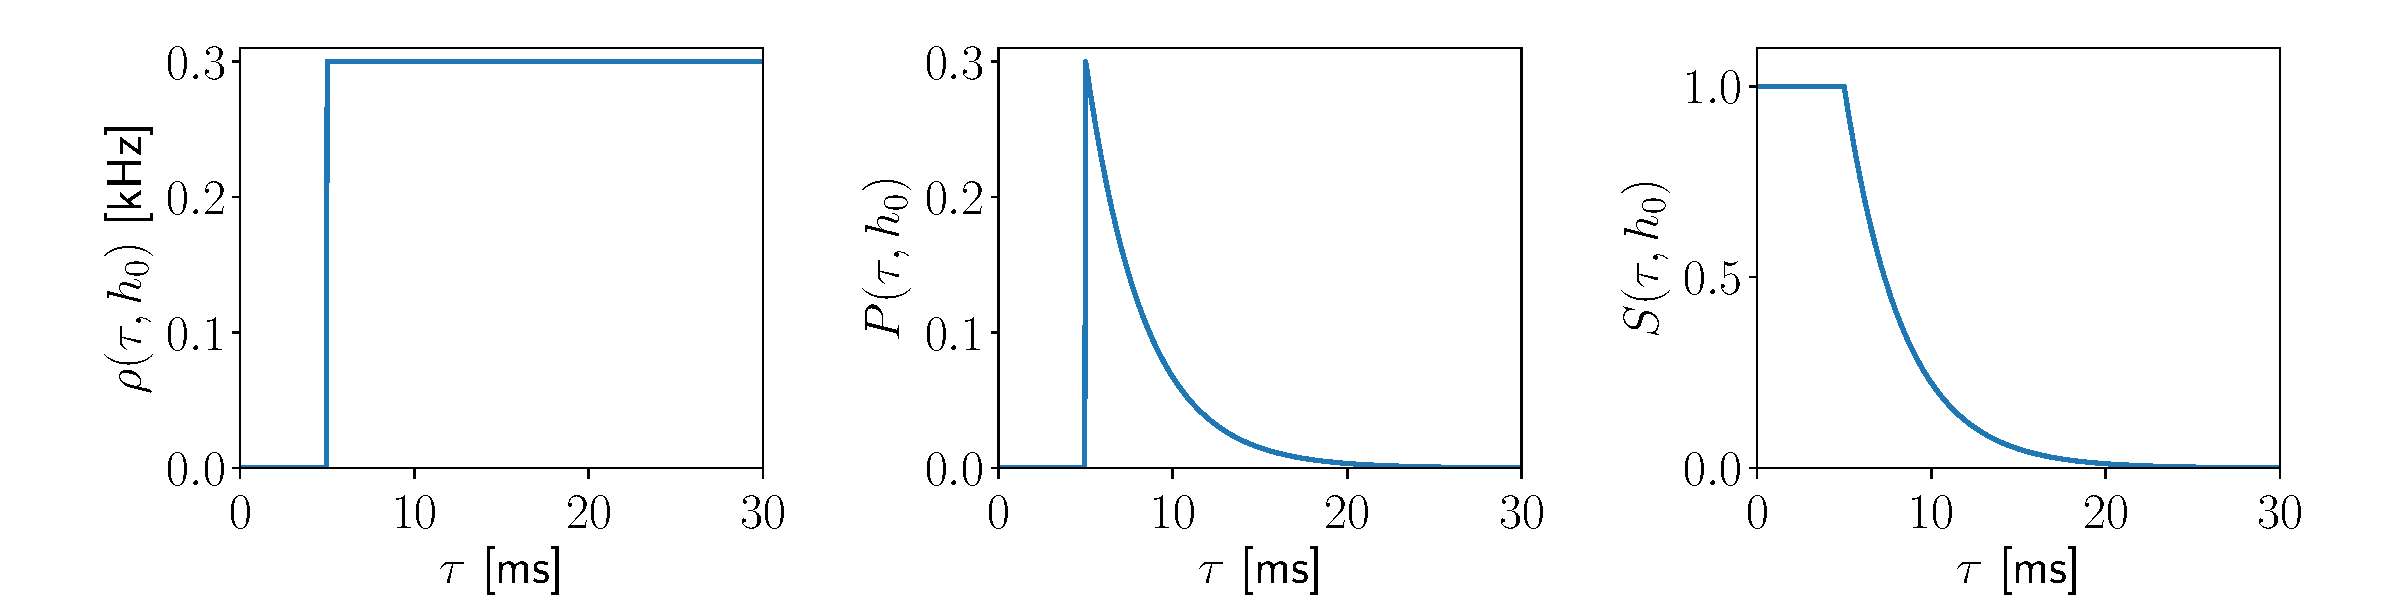
\includegraphics[width=\linewidth]{poissonRHOSP.pdf}
	(b)\\
	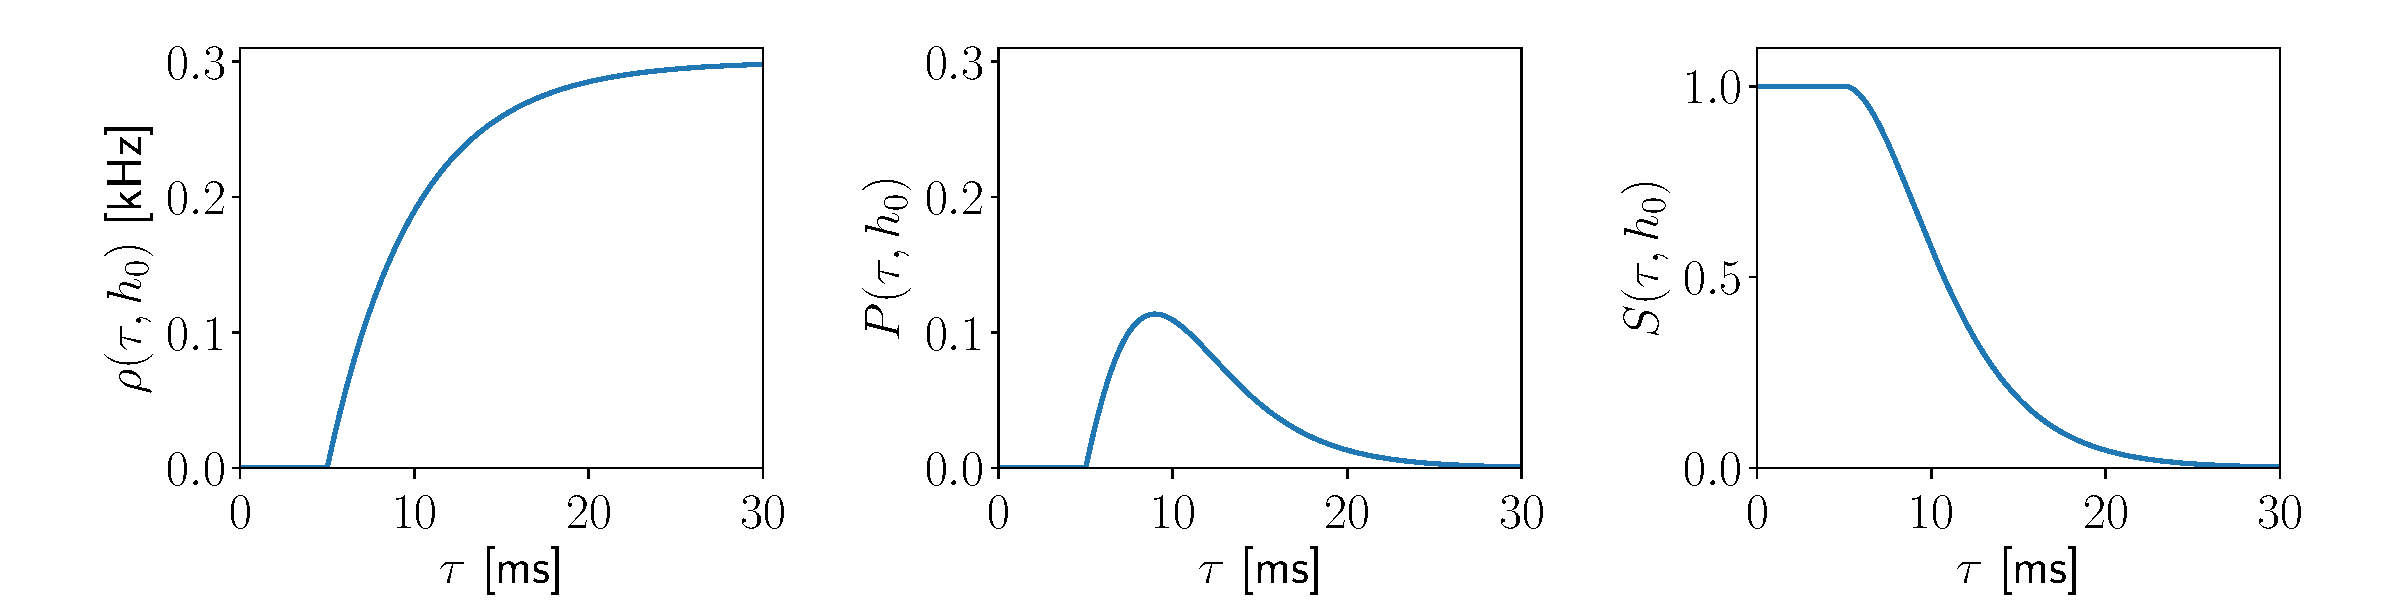
\includegraphics[width=\linewidth]{expRHOSP.pdf}
	\caption{Hazard rate $\rho(\tau,h)$ (left), interval distribution $P(\tau,h)$ (middle) and survivor function $S(\rho(\tau,h)$ (right) for different recovery function $g(\tau)$. (a) Recovery function corresponds to a Poisson neuron with absolute refractoriness $\Delta$, with $Delta=10$ ms, $h=h_0$, $\nu_{max}=100$ Hz.  (b) Recovery function defined  by $ g(\tau)=\left[1-\exp(-\lambda(\tau-\Delta))\right]\theta(\tau-\Delta)$ Poisson neuron with absolute refractoriness $\Delta$, with $\Delta=10$ ms, $h=h_0$, $\nu_{max}=100$ Hz.  }
	\label{fig:renewalprocess}
\end{figure}


\paragraph{Gamma process}

The gamma process is often used to model spike trains as it is one of the easiest non-Poisson process to analyze. The interspike distribution is given by:

\begin{equation}
\label{eq:gamma}
P(\tau)=\frac{\beta^\gamma}{\Gamma(\gamma)}\tau^{\gamma-1}e^{-\beta\tau}
\end{equation}

The rate of this process  is $R=\beta/\gamma$, And the coefficient of variation is given by $C_V=\gamma^{-\frac{1}{2}}$. For $\gamma=1$ this corresponds to a Poisson process. For $C_V>1$ the Interspike distributiondiverges as $\tau$ goes to $0$. If gamma is an integer, one can see the gamma process as a chain of $\gamma$ poisson neuron with rate $\beta$ before, this implies that the global rate of the total chain is $R=\beta/\gamma$, and induces refractoriness as shown on Fig.\ref{fig:gammaprocess}


\begin{figure}
	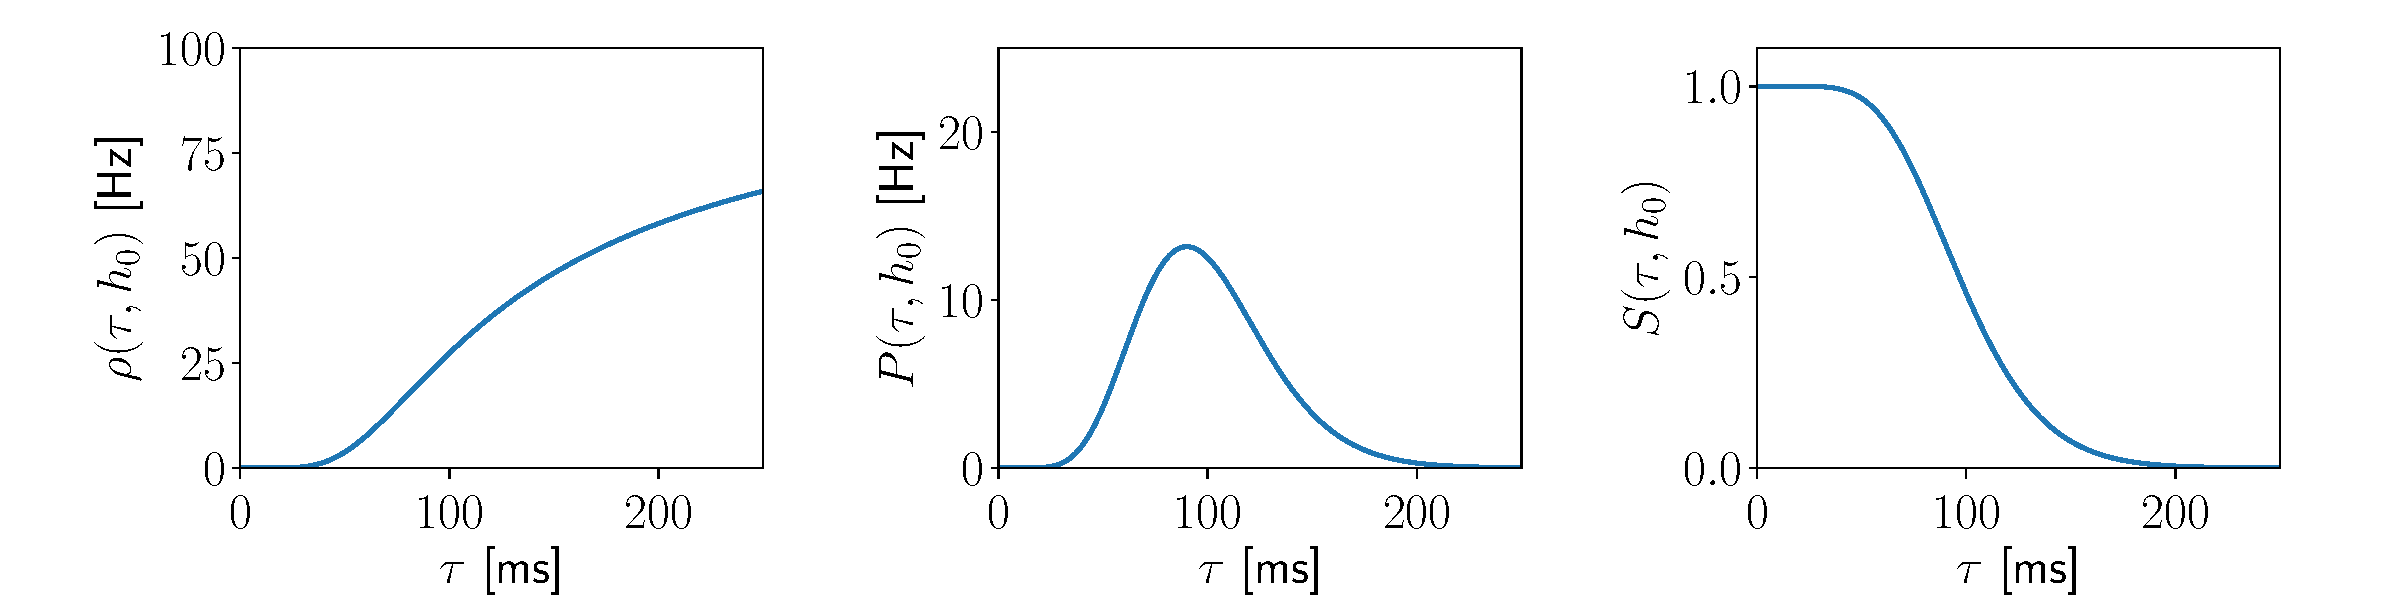
\includegraphics[width=\linewidth]{gamma.pdf}
	\caption{Hazard rate $\rho(\tau)$ (left), interval distribution $P(\tau)$ (middle) and survivor functio $S(\rho(\tau)$ (right) for a Gamma Process with $\beta=100$ Hz
		$\gamma=10$ }
	\label{fig:gammaprocess}
\end{figure}

\paragraph{Perfect integrate-and-fire model driven by white noise}
\label{sec:pif}
The perfect integrating-and fire model has been used  to explain statistics of of single neuron. The membrane potential can be seen as a Browmian-motion with drift $\mu$ (mean current) driven by a white noise


\begin{align}
\label{eq:Vxi}
\dot V=\mu +\sqrt{2D}\xi(t), \:\:\:\:\:\:\:\: \:\:\:\:\: if\:\:\:\:\:\:  V=V_{th}\:\:\:\:\:\:V\rightarrow V_r\\ 
<\xi(t)\xi(s)>=\delta(t-s)
\end{align}

\begin{figure}
	\centering
	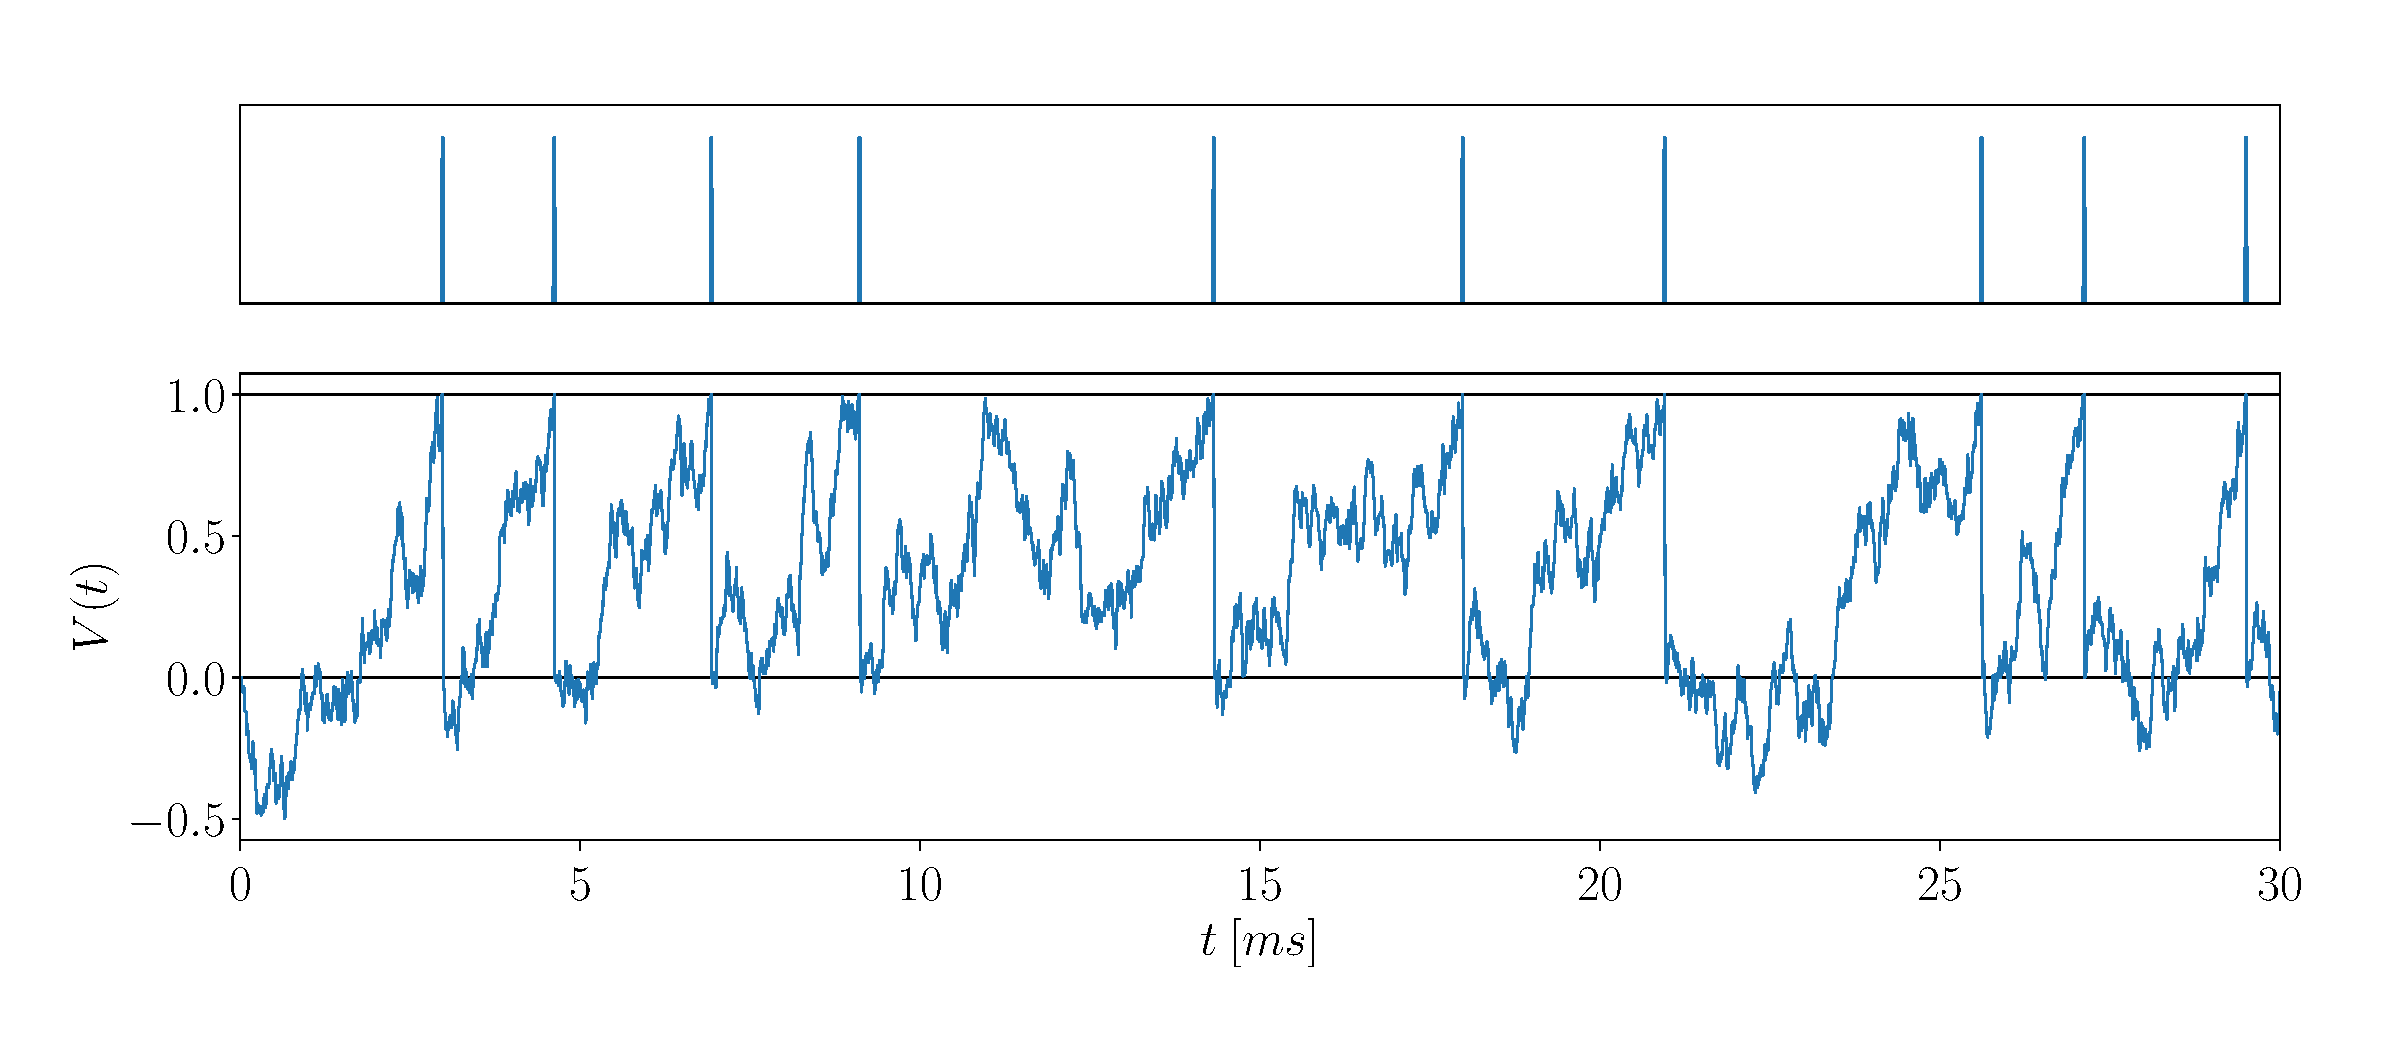
\includegraphics[width=0.8\linewidth]{PIF_V}
	\caption{Typical realization $V(t)$ for the PIF model driven with a white noise with $\mu=0.3$ $V_{th}$ kHz, $D=0.1$ $V_{th}^2$ kHz, $V_{th}=1$. The generated spike train is indicated on the top.
	}
	\label{fig:PIF_V}
\end{figure}


\begin{figure}
	
	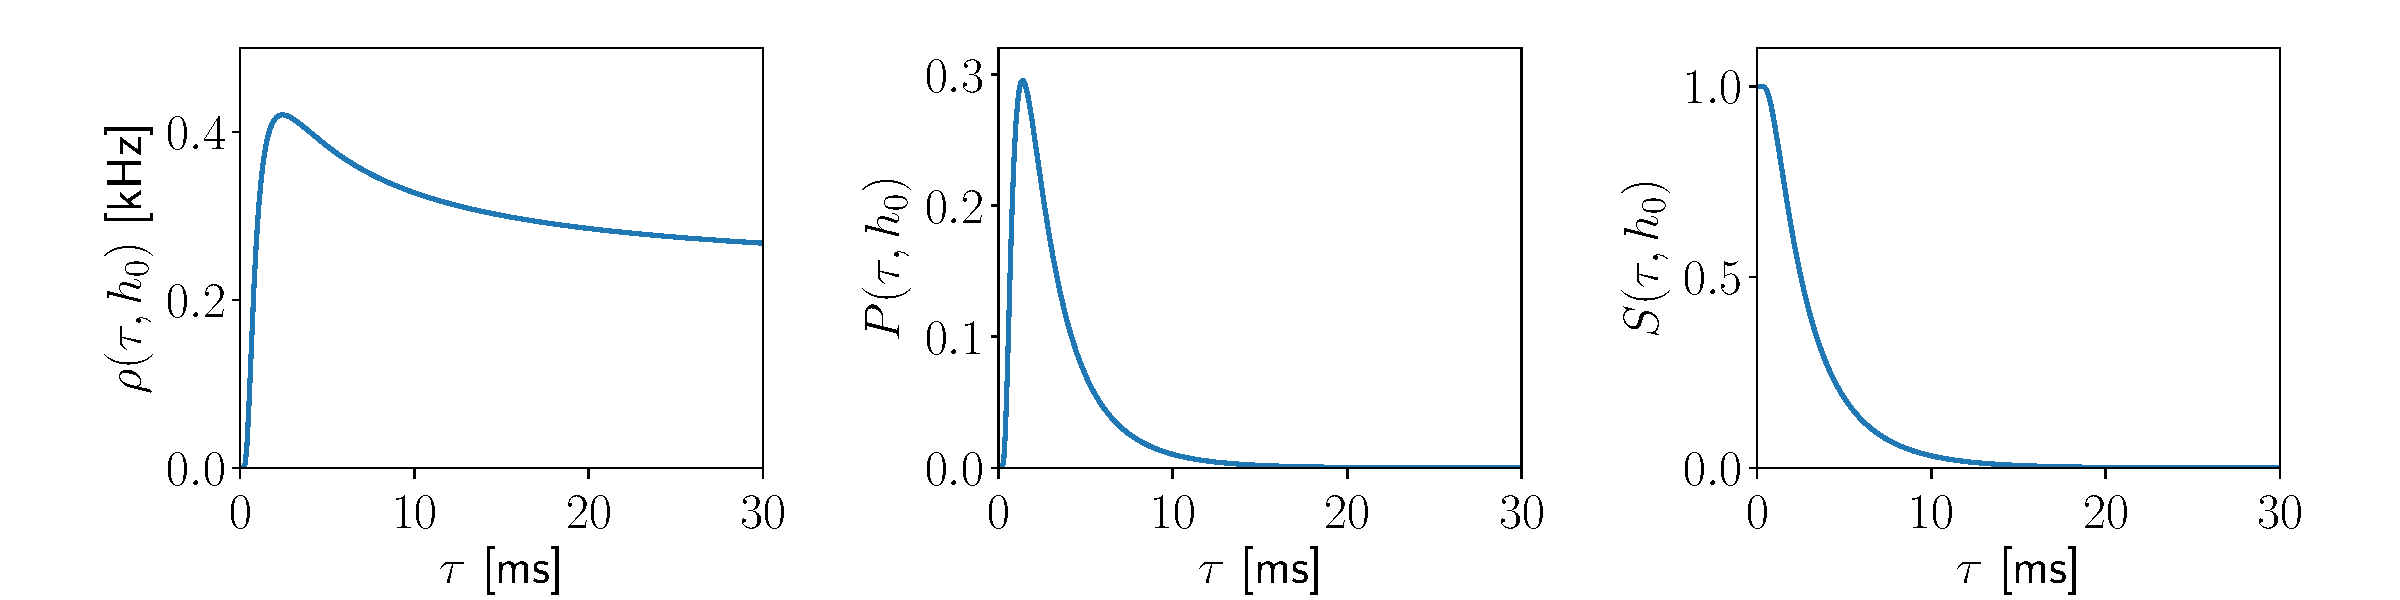
\includegraphics[width=\linewidth]{inversegaussian.pdf}
	\caption{Hazard rate $\rho(\tau)$ (left), interval distribution $P(\tau)$ (middle) and survivor functio $S(\rho(\tau)$ (right) for the PIF model.
	}
	\label{fig:inversegaussianprocess}
\end{figure}



\subsection{Populations of neurons and refractory density equations}

\subsubsection{Network model}

There are more than 86 billion neurons in the brain, distributed in different brain area and which form elaborate neural networks. Within a brain area one can identify subregions and layers where neurons are organize in populations of cells with similar property. Given the large number of neurons in a population, rather than track the spiking of individual neurons, instead it is appealing to describe the mean activity. 
Those theory of population dynamics date back to the 1970s (todo ref)and are still widely use to predict the temporal evolution of the activity $A(t)$. In a network of N neurons the population activity $A(t)$ is defined as the proportion of active neuron:
\begin{equation}
A(t)=\frac{1}{N}\sum_{j=1}^N\sum_f\delta(t-t_j^f)
\end{equation}

where $\delta$ denotes the dirac function ad the double sum runs over all firing time $t^f$ of all neuron $j$ in the population.

We consider large homogeneous population of neurons i.e all neuron are identical and receive the same external input


 



- population activity definition

- definition of network : all-to-all coupling

-external input $\mu(t)$
\begin{equation}
\label{eq:mu}
\mu(t)=V_{rest}+RI_{ext}(t)+RI_{syn}(t)
\end{equation}

- and/or synaptic input
\begin{equation}
\label{eq:input}
RI_{syn}(t)=\tau_mJA(t)
\end{equation}

\subsubsection{Refractory density equation}

An approach on the refractory density $q(\tau,t) $ can be used to analyze the dynamic in a neuron network. $q(\tau,t)$ defined the density of neuron at time $t$ with age $\tau=t-\hat{t}$ where $\hat{t}$. The activity of a network is thus given by
\begin{equation}
\label{eq:A}
A(t)=q(0,t)
\end{equation}

As long as a neuron does not fire, the age $\tau$ increase at the speed of $\frac{\dd \tau}{\dd t}=1$, therefore the flux along the refractory variable $\tau$ is simply $q(\tau,t)$ and the continuity equation  is given by

\begin{equation}
\label{eq:continuity1}
\frac{\partial q}{\partial t}=-\frac{\partial q}{\partial \tau}
\end{equation}

When a neuron fires, the trajectory along the refractory variable $\tau$ stops at the current value and "reappears" at $\tau=0$. The instantaneous probability to fire is given by the hazard function.Therefore the loss per unit time is given by $-\rho(\tau,h)q()\tau,t)$ and the full dynamic is then given by the master equation:

\begin{equation}
\label{eq:masterequation}
\partial_t q(\tau,t)=-\partial_\tau q(\tau,t)-\rho(\tau,h)q(\tau,t)
\end{equation}

The dynamics is schematize on Fig.\ref{fig:qtau}. At time $t_j$ The proportion of neurons at age $\tau_i$ whose are firing and will reappear at age $0$, is given by$q(\tau_i,\tau_j)\rho(\tau_i,h_j)\Delta t$ (red arrow). The neuron whose did not fire will reach the age $\tau_{i+1}$ at time $t_{j+1}$ (Blue arrow). The sum of all trajectory that "disappear" at time $t$ due to firing, are "reappearing" at $\tau=0$ and  neuron will fire at some finite time, therefore the boundary condition are:

\begin{align}
\label{eq:boundarycondition}
q(0,t)&=\int_{0}^{\infty}\rho(\tau,h)q(\tau,t)d\tau=A(t) \\
q(\infty,t)&=0
\end{align}

Additionally, $q$ is normalized

\begin{equation}
\label{eq:qnormalisation}
\int_0^\infty q(\tau,t)\dd \tau = 1
\end{equation}

and has the initial density

\begin{equation}
\label{eq:qinitial}
q(\tau,0)=q_0(\tau)
\end{equation}

where $q_0(\tau)$ is some function that satisfies the conditions Eq.\eqref{eq:boundarycondition},\eqref{eq:qnormalisation}


\cite{Ger00,ChiGra07}


\begin{figure}
	\centering
	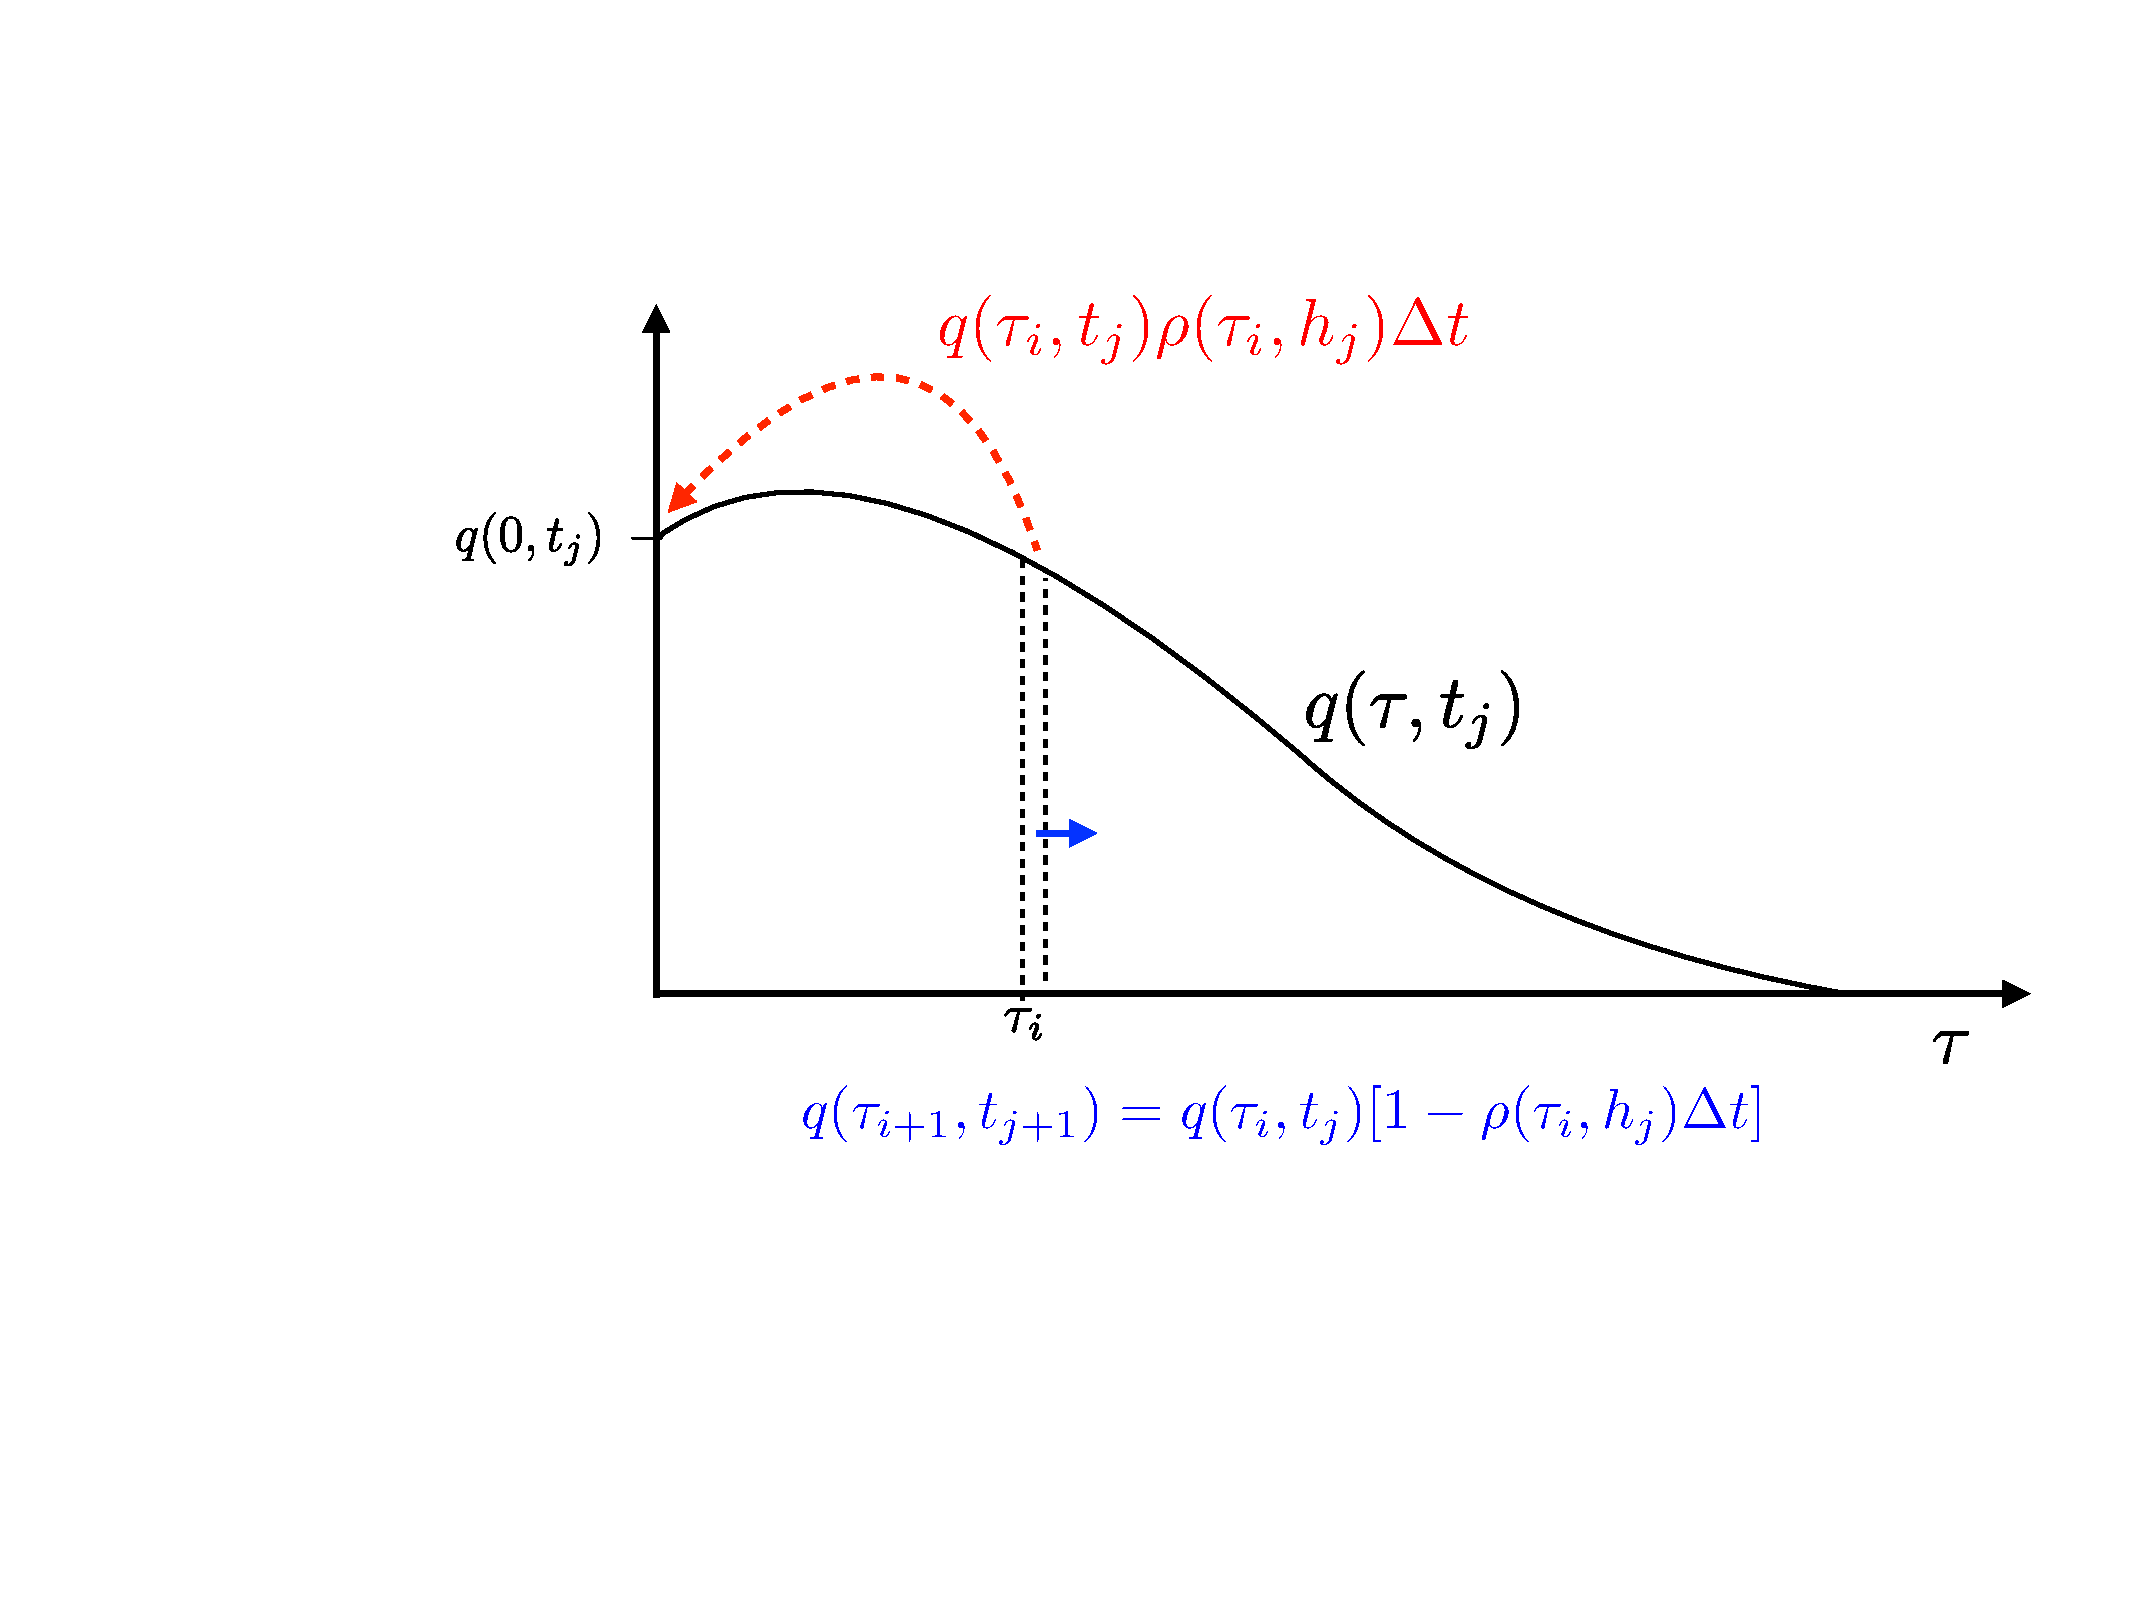
\includegraphics[width=0.7\linewidth]{qtau.pdf}
	\caption{Scheme of refractory density dynamics. The red arrow represents the proportion of neurons with age $\tau_i$ whose fire at time $t_j$, the blue one represents those that are not firing and will reach the age $\tau_{j+1}$ at time $t_{j+1}$
	}
	\label{fig:qtau}
\end{figure}



\subsection{Spectral decomposition method}

The  eigenfunction expansion is a method applied on partial differential equation. The main idea is identify an operator and expand the equation in terms of the operator eigenfunction times time dependent coefficient. 


For concreteness, and to recall the basic property of this methods, we will introduce the spectral expansion of the Fokker-Planck operator.


\subsubsection{Spectral decomposition of the Fokker-Planck equation}
An approach on the membrane potential densities $p(v,t)$ can be used to analyse the dynamics of networks of integrate and fire neurons. We assume that a neuron can be described by one state variable e.g. the membrane potential $v$.

For a large homogeneous network of IF neurons, the evolution of probability density function $p(v,t)$ is described by the Fokker-Planck equation (TODO add reference).  

\begin{equation}
\label{eq:fokkerplanck}
\partial_t p(v,t)=\mathcal{L}p(v,t)
\end{equation}

where $\mathcal{L}$ is the Fokker-Planck operator, which takes the general form

\begin{equation}
\label{eq:Lfokker}
\mathcal{L}(v,t)=-\partial_v A(v,t) +\partial_v^2 B(v,t)
\end{equation}

The Fokker-Planck operator is in general non linear because it depend on activity $A(t)$ given by the flux of realizations crossing the emission threshold $\theta$.


\subsubsection{General properties of the Fokker-Planck operator}
The Fokker-Planck operator has a set of eigenfunctions and associated eigenvalues:
\begin{equation}
\label{eq:fokkerplanckoperator}
\mathcal{L}\ket{\phi_n}=\lambda_n\ket{\phi_n}
\end{equation}

If the eigenvalues $\lambda_n$ are complex, the complex conjugate of an eigenvalue  $\bar{\lambda}_n$  is also an eigenvalue of $\mathcal{L}$, with eigenfunction $\ket{\bar{\phi_n}}$ because $\mathcal{L}$ is a real operator. We will use the notation $\bar{\lambda}_n=\lambda_{-n}$, so that the sums over the spectrum of $\mathcal{L}$ range over all integer numbers. Note that $\lambda_0=0$ is always an eigenvalue of the operator $\mathcal{L}$ and corresponds to the stationary solution.

Because $\mathcal{L}$ cannot be generally brought to an Hermitian form we also need  the eigenfunction $\ket{\psi_n}$ of the adjoint operator  $\mathcal{L}^{+}$

\begin{equation}
\label{eq:fokkerplanckoperatordega}
\mathcal{L}^+\ket{\psi_n}=\tilde{\lambda}_n\ket{\psi_n}
\end{equation}

Defining the inner product one can show that the eigenvalues of Eq.\eqref{eq:fokkerplanckoperator} and Eq.\eqref{eq:fokkerplanckoperatordega} are the same:

\begin{equation}
\label{eq:innerproduct}
\langle\psi|\phi\rangle=\int\psi(v,t)\phi(v,t)dv
\end{equation}

\begin{align}
\lambda_n\langle\psi_n|\phi_n\rangle &=\int\psi(v,t)\mathcal{L}\phi(v,t)\dd v  \nonumber \\
&=\langle\psi_n|\mathcal{L}\phi_n\rangle \nonumber \\
&=\langle\mathcal{L}^+\psi_n|\phi_n\rangle  \nonumber \\
&=\int\mathcal{L}^+\psi_n(v,t)\phi_n(v,t)\dd v \nonumber \\
&=\tilde{\lambda}_n\langle\psi_n,|\phi_n\rangle \label{eq:sameeig}
\end{align}

Eq.\eqref{eq:sameeig} implies that $\lambda_n=\tilde{\lambda}_n$ and

\begin{equation}
\label{eq:fokkerplanckoperatordega2}
\mathcal{L}^+\ket{\psi_n}=\lambda_n\ket{\psi_n}
\end{equation}


For different eigenvalues, the eigenfunctions $\psi_i$ and $\phi_j$ are orthogonal

\begin{align}
\lambda_j\langle\psi_i|\phi_j\rangle
&=\langle\psi_i|\mathcal{L}\phi_j\rangle \nonumber \\
&=\langle\mathcal{L}^+\psi_i|\phi_j\rangle  \nonumber \\
&=\lambda_i\langle\psi_i|\phi_j\rangle \label{eq:lorthogonal}
\end{align}

And with an appropriate normalization the two set of eigenfunctions are biorthonormal

\begin{equation}
\label{eq:dij}
\langle\psi_i|\phi_j\rangle=\delta_{ij}
\end{equation}



\subsection{Expansion and rate equation}
The spectrum $\{\lambda_n\}$ of the Fokker-Planck operator provide a moving basis $ \{\ket{\phi_n}\}$. The density $p(v,t)$ can be expressed in terms of this basis

\begin{equation}
\label{eq:p}
\ket{p}=\sum_na_n\ket{\phi_n}
\end{equation}

where $a_n=\langle \psi_n | p\rangle$ are the time dependent coefficients of the modal expansion. Since $p$ is real $\bar{a}_n=a_{-n}$. The dynamics of the $a_n$ can be determined directly from the Fokker-Plank equation

\begin{align}
\dot{a}_n&=\langle\psi_n|\partial_t p\rangle+\langle\partial_t\psi_n|p\rangle \nonumber \\
&=\langle\psi_n|\mathcal{L}p\rangle+  \dot{\nu}\sum_ma_m\langle\partial_\nu\psi_n|\phi_m \rangle \nonumber \\
&=\lambda_n a_n +  \dot{\nu}\sum_ma_m\langle\partial_\nu\psi_n|\phi_m \rangle \nonumber \\
\end{align}

Here we have use the fact that the time dependence of $\psi$ is due to the moment of $\nu$. An emission rate equation result

\begin{align}
\dot{\vec{a}}&=(\boldsymbol{\Lambda}+\boldsymbol{C}\dot{h})\vec{a}+\vec{c}\dot{h}\nonumber\\
\nu&=\Phi+\vec{f}\cdot\vec{a}
\end{align}

where $\nu(t)$ is the instantaneous firing rate. $\vec{a}=\{a_n\}_{n \neq 0}$. $\vec{f}$ are the flux in $\theta$ for non stationary modes. The synamptic coupling are expressed in the in the vector $\vec{c}$ $c_n=\langle\partial_h\psi_n|\phi_0\rangle$, $\forall n \neq 0$ and the matrix $\boldsymbol{C}$: $C_{nm}=\langle\partial_h\psi_n|\phi_m\rangle$ , $\forall n \neq 0$. And $\boldsymbol{\Lambda}$ is the diagonal matrix of the eigenvalues of $\mathcal{L}$: $\Lambda_{nm}=\lambda_n\delta_{nm}$





\section{Theory}
\label{sec:theory}
\subsection{Operator of the refractory density, and eigenvalue spectrum $\{\lambda_n\}$}

The master equation Eq.\eqref{eq:masterequation} can be rewritten introducing the operator :

\begin{equation}
\label{eq:Loperator}
\mathcal{L}=-\partial_\tau-\rho(\tau,h)
\end{equation}

\begin{equation}
\label{eq:masterequation2}
\partial_t q(\tau,t)=\mathcal{L}q(\tau,t)
\end{equation}

The set of eigenfunctions and associated eigenvalues of $\mathcal{L}$ obeys to
\begin{equation}
\label{eq:Loperator2}
\mathcal{L}\ket{\phi_n}=\lambda_n\ket{\phi_n}
\end{equation}

And respect the boundary conditions Eq.\eqref{eq:boundarycondition}

\begin{align}
\label{eq:boundarycondition2}
\phi_n(0,h)&=\int_0^\infty\rho(\tau,h)\phi_n(\tau,h)\dd\tau\\
\phi_n(\infty,h)&=0\\
\end{align}


 To lighten the notation, we omit the dependence on $h$ (the time dependent parameter) of the hazard rate $\rho(\tau)$, The ISI distribution $P(\tau)$, the surivor funtion $S(\tau)$, and of the set of eigenfunctions $\{\ket{\phi_n}\}$ and eigenvalues $\{\lambda_n\}$.

The solution of Eq.\eqref{eq:Loperator2} is

\begin{align}
\label{eq:phin}
\phi_n(\tau)&=\phi_n(0)\exp(-\lambda_n\tau-\int_0^\tau\rho(s)ds)\nonumber\\
&=\phi_n(0)e^{-\lambda_n\tau}S(\tau)
\end{align}

Inserting the Eq.\eqref{eq:phin} in the boundary condition Eq.\eqref{eq:boundarycondition2}, we find the condition

\begin{equation}
\label{eq:condition1}
\phi_n(0)=\int_0^\infty\rho(\tau)\phi_n(0)\exp(-\lambda_n\tau-\int_0^\tau\rho(s)ds)\dd\tau
\end{equation}

which can be written as

\begin{equation}
\label{eq:condition2}
1=\int_0^\infty e^{-\lambda_n \tau}P(\tau)dd\tau=P_L(\lambda_n)\\
\end{equation}

The condition Eq.\eqref{eq:condition2} was already derived by Tilo Schwalger in an unpublished paper. It states that the Laplace transform of the ISI density $P_L(\lambda)$ at the (complex) arguments $\lambda_{n}$ must be unity. 

We can conclude some properties of the spectrum {$\lambda_n$} imposed by Eq.\eqref{eq:condition2}

As expected, the eigenvalue $\lambda_0=0$ fulfilled the condition because the ISI density is normalized. This eigenvalue corresponds to the stationary density.

The real part of $\lambda_n$ cannot be positive, as expected for physical reason. Indeed the solution of the refractory density equation is directly related to the eigenvalues of $\mathcal{L}$ and is expected to converge to $\phi_0$, instead of exploding which would be the case for positive eigenvalues. In fact fo $\Re(\lambda_n)>0$,

\begin{equation}
\int_0^\infty e^{-\lambda_n \tau} P(\tau) \dd\tau<\int_0^\infty |e^{-\lambda_n\tau} |P(\tau) \dd\tau<\int_0^\infty P(\tau) \dd\tau=1
\end{equation}

which contradict Eq.\eqref{eq:condition2}.



\subsection{Adjoint operator $\mathcal{L}^+$, and normalization}

Because $\mathcal{L}$ cannot be generally brought to an Hermitian form we also need  the eigenfunction $\psi_n$ of the adjoint operator  $\mathcal{L}^{+}$

\begin{equation}
\label{eq:Ldegaoperator}
\mathcal{L}^+\ket{\psi_n}=\lambda_n\ket{\psi_n}
\end{equation}

We can find the adjoint operator $\mathcal{L}$, using the integration by part

\begin{align}
\langle\psi|\mathcal{L}\phi\rangle&= \int_{0}^{\infty}\psi(\tau)\mathcal{L}\phi(\tau)\dd\tau  \nonumber \\
&= \int_{0}^{\infty}\psi(\tau)[-\partial_{\tau}-\rho(\tau)]\phi(\tau)\dd\tau  \nonumber \\
&=-[\psi(\tau)\phi(\tau)]^{\infty}_{0}+\int_{0}^{\infty}\partial_{\tau}\psi(\tau)\phi(\tau)\dd\tau -\int_{0}^{\infty}\rho(\tau)\psi(\tau)\phi(\tau)\dd\tau \nonumber \\
&= \psi(0)\phi(0)+ \int_{0}^{\infty}[\partial_{\tau}-\rho(\tau)]\psi(\tau)\phi(\tau)\dd\tau  \nonumber \\
&=\int_{0}^{\infty} \psi(0)\rho(\tau)\phi(\tau)\dd\tau+ \int_{0}^{\infty}[\partial_{\tau}-\rho(\tau)]\psi(\tau)\phi(\tau)\dd\tau  \nonumber \\
&= \int_{0}^{\infty}\big\{[\partial_{\tau}-\rho(\tau)]\psi(\tau)+ \psi(0)\rho(\tau)\big\}\phi(\tau)d\tau  \nonumber \\
& = \langle\mathcal{L}^+\psi|\phi\rangle
\end{align}


As we will normalize the eigenfunction to obtain a biorthonormal basis we can set $\psi(0,h)=1$, and the adjoint operator can be express as

\begin{equation}
\label{eq:Ldega}
\mathcal{L}^+\psi(\tau,h)=[\partial_{\tau}-\rho(\tau)]\psi(\tau)+\rho(\tau)
\end{equation}

The solution of Eq.\eqref{eq:Ldegaoperator} is

\begin{align}
\label{eq:psin}
\psi_n(\tau)&=\exp\big(\lambda_n\tau+\int_0^\tau\rho(s)ds\big)\nonumber\big[1-\int^\tau_0 \rho(x) \exp\big(-\lambda_nx-\int_0^x\rho(s)ds\big)dx\big]\\
&=e^{\lambda_n\tau}S^{-1}(\tau)\big[1-\int^\tau_0 P(x) e^{-\lambda_nx}dx\big]
\end{align}

In particular we have

\begin{align}
\label{eq:psi0}
\psi_0(\tau)=1
\end{align}



The a biorthonormal basis is obtained inserting Eq.\eqref{eq:phin} and Eq.\eqref{eq:psin} in Eq.\eqref{eq:dij}, teh normalization is then given by 

\begin{align}
1=&\int_0^{\infty}\phi_n(0)\big[1-\int^\tau_0 P(x) \exp\big(-\lambda_nx)dx\big]d\tau \\
\phi_n(0) =&\frac{1}{\int_0^{\infty}\big[1-\int^\tau_0 P(x) e^{-\lambda_nx}dx\big]d\tau}
\end{align}


In particular for $n=0$, $\lambda_0=0$ and we recover the relation:

\begin{equation}
\phi_0(0) = \frac{1}{\int_0^{\infty}S(\tau)d\tau}
\end{equation}

\subsection{Emission rate equation}

As the density $p(v,t)$ with the Fokker-Planck equation, the refractory density $q(tau,t)$ can be expressed in the eigenfunction  $ \{\ket{\phi_n}\}$. T

\begin{equation}
\label{eq:q}
\ket{q}=\sum_na_n\ket{\phi_n}
\end{equation}

where $a_n=\langle \psi_n | q\rangle$ are the time dependent coefficients of the modal expansion. In particular from Eq.\eqref{eq:psi0}, and Eq.\eqref{eq:dij} we have $a_0(t)=1$. The dynamics of the $a_n$ can be determined directly using Eq.\eqref{eq:Loperator}, and Eq.\eqref{eq:masterequation2}

\begin{align}
\dot{a}_n&=\langle\psi_n|\partial_t q\rangle+\langle\partial_t\psi_n|q\rangle \nonumber \\
&=\langle\psi_n|\mathcal{L}q\rangle+  \dot{h}\sum_ma_m\langle\partial_h\psi_n|\phi_m \rangle \nonumber \\
&=\lambda_n a_n +  \dot{h}\sum_ma_m\langle\partial_h\psi_n|\phi_m \rangle 
\end{align}

Defining the coupling coefficient as $C_{nm}=\langle\partial_h\psi_n|\phi_m \rangle $ we can rewrite

\begin{equation}
\dot{a}_n=\lambda_n a_n +  \dot{h}\sum_mC_{nm}a_m 
\end{equation}



We can finally express the activity $A(t)=q(0,t)$ as

\begin{equation}
\label{eq:A2}
A(t)=\sum_na_n(t)\phi_n(0)
\end{equation}

Keeping only the first mode, and using the fact that $\ket{\phi_{-n}}=\ket{\bar{\phi}_n}$ and $a_{-n}=\bar{a}_n$,  Eq.\eqref{eq:A2} become

\begin{align}
\label{eq:A3}
A(t)&=\phi_0(0) + a_1\phi_1(0) +a_{-1}\phi_{-1}(0) \nonumber \\
      &=\phi_0(0) + 2\big[\Re\big(a_1\big)\Re\big(\phi_1(0)\big)- \Im\big(a_1\big)\Im\big(\phi_1(0)\big)\big] 
\end{align}


And the dynamics of the $a_1$ is given by
\begin{equation}
\label{eq:a1}
\dot{a}_1=\lambda_1 a_1 + \dot{h}\big[C_{10}+C_{11}a_1+C_{1-1}a_{-1}\big] \nonumber \\
\end{equation}

Separating explicitly the real part $X(t)$ and the imaginary part  $Y(t)$ of $a_1(t)$

 \begin{equation}
 \label{eq:a1xy}
 a_1(t)= X(t) +i Y(t)
 \end{equation}
 
 we derived from Eq.\eqref{eq:a1}  two non linear differential equation

\begin{align}
\dot{X}(t)=&\Re[f]X(t)-\Im[g]Y(t) +\Re[C_{10}]\dot{h}\\
\dot{Y}(t)=&\Re[g(h)]Y(t)+\Im[f(h)]X(t) +\Im[C_{10}]\dot{h}\\
\end{align}

with
\begin{align}
f(h)=&\lambda_1+ \dot{h}(c_{11}+c_{1-1})\\
g(h)=&\lambda_1+ \dot{h}(c_{11}-c_{1-1})
\end{align}

We have finally a set of three non linear differential equation $\dot{h}(t)$, $\dot{X}(t)$, $\dot{Y}(t)$


\section{Spectrum}
\subsection{Spectral derivation for specific model}
\label{sec:specif-model}


\subsubsection{Poisson neuron with absolute refractoriness}
\label{subsec:absref}


In this section we will consider a Poisson neuron with absolute refractoriness $\Delta$, the hazard rate is defines by the recovery function Eq.\eqref{eq:poissonabs}.
To simplify the notation we will use the variable $\nu$ such that $\nu=\Phi(h)$. The hazard rate is then given by

\begin{equation}
\rho(\tau)=\nu\:\Theta(\tau-\Delta)
\end{equation}


And the interspike interval distribution is 
\begin{equation}
P(\tau)=\nu \Theta(\tau-\Delta) \exp\big(-\nu(\tau-\Delta)\big)
\end{equation}


%\be
%S(\tau)=\Theta(\Delta-\tau) +  \Theta(\tau-\Delta) \exp(-\nu(\tau-\Delta))
%\ee

For this process we can compute the Laplace transform of the ISI density

\begin{align}
P_L(\lambda)=&\int_0^\infty P(\tau)e^{-\lambda \tau}\nonumber\\
=&\frac{\nu}{\nu+\lambda}exp(-\lambda \Delta)
\end{align}
%=&\int_\Delta^\infty \nu \exp\big(-(\lambda+\nu)\tau)\big)\exp\big(\nu \Delta\big)\\


By the change of variable $w=(\nu+\lambda_n)\Delta$, the condition Eq.\eqref{eq:condition2}, can be rewriten as

%\frac{\nu}{\nu+\lambda}exp(-\lambda_n \Delta)=1

\begin{equation}
\label{eq:weq}
\Delta \nu e^{\nu\Delta}=we^{w} 
\end{equation}

The solution of equation Eq.\eqref{eq:weq} is given introducing the Lambert W-function $W(z,n)$
\begin{equation}
w=W(\Delta \nu e^{\nu\Delta},n)
\end{equation}

from which we read the eigenvalue spectrum $\{\lambda_n\}$

\begin{equation}
\lambda_n=\frac{1}{\Delta}W(\Delta \nu e^{\nu\Delta},n) - \nu
\end{equation}


We can explicitly express the eigenfunctions, $\ket{\phi_n}$ of the operator $\mathcal{L}$ and $\ket{\psi_n}$ of  the adjoint operator $\mathcal{L}^+$

%\begin{align}
%\phi_n(0) =&\frac{1}{\int_0^{\infty}\big[1-\int^\tau_0 \nu \Theta(x-\Delta) \exp(-\nu(x-\Delta)) \exp\big(-\lambda_nx)dx\big]d\tau}\\
%=& \frac{\nu+\lambda_n}{1+\Delta(\nu+\lambda_n)}
%\end{align}

\begin{equation}
\phi_n(\tau)= \frac{\nu+\lambda_n}{1+\Delta(\nu+\lambda_n)}\exp(-\lambda_n\tau)\big[\Theta(\Delta-\tau) +  \Theta(\tau-\Delta) \exp(-\nu(\tau-\Delta))\big]
\end{equation}


\begin{align}
\psi_n(\tau)=&\Theta(\Delta-\tau)\exp(\lambda_n\tau) +  \Theta(\tau-\Delta) \frac{\nu}{\nu+\lambda_n}\\
=&\Theta(\Delta-\tau)\exp(\lambda_n\tau) +  \Theta(\tau-\Delta) \exp(\lambda_n\Delta)\\
\end{align}



In order to define the coupling coefficient we need first to compute $\frac{d\psi_n(\tau)}{d\nu}$ 
\begin{equation}
\frac{\partial\psi_n(\tau)}{\partial\nu}=\frac{\lambda_n}{\nu[1+\Delta(\nu+\lambda_n)]}\big[\Theta(\Delta-\tau)\tau\exp(\lambda_n\tau) +  \Theta(\tau-\Delta)\Delta \exp(\lambda_n\Delta)\big]\\
\end{equation}

The coupling coefficient are then 

\begin{align}
C_{nn}=&\frac{\partial \nu}{\partial h}\int_0^\infty\frac{d\psi_n(\tau)}{d\nu}\phi_n(\tau)d\tau \nonumber\\
=&\frac{\lambda_n\Delta(1+\frac{1}{2}\lambda_n(\nu+\lambda_n))}{\nu(1+\Delta(\nu+\lambda_n))}\frac{\partial \nu}{\partial h}
\end{align}


\begin{align}
C_{nm}=&\frac{\partial \nu}{\partial h}\int_0^\infty\frac{d\psi_n(\tau)}{d\nu}\phi_m(\tau)d\tau \nonumber\\
=&\frac{\lambda_n(\nu+\lambda_m)}{\nu(\lambda_n-\lambda_m)(\nu+\lambda_n)(1+\Delta(\nu+\lambda_m))}\frac{\partial \nu}{\partial h}
\end{align}


\begin{figure}
	\centering
	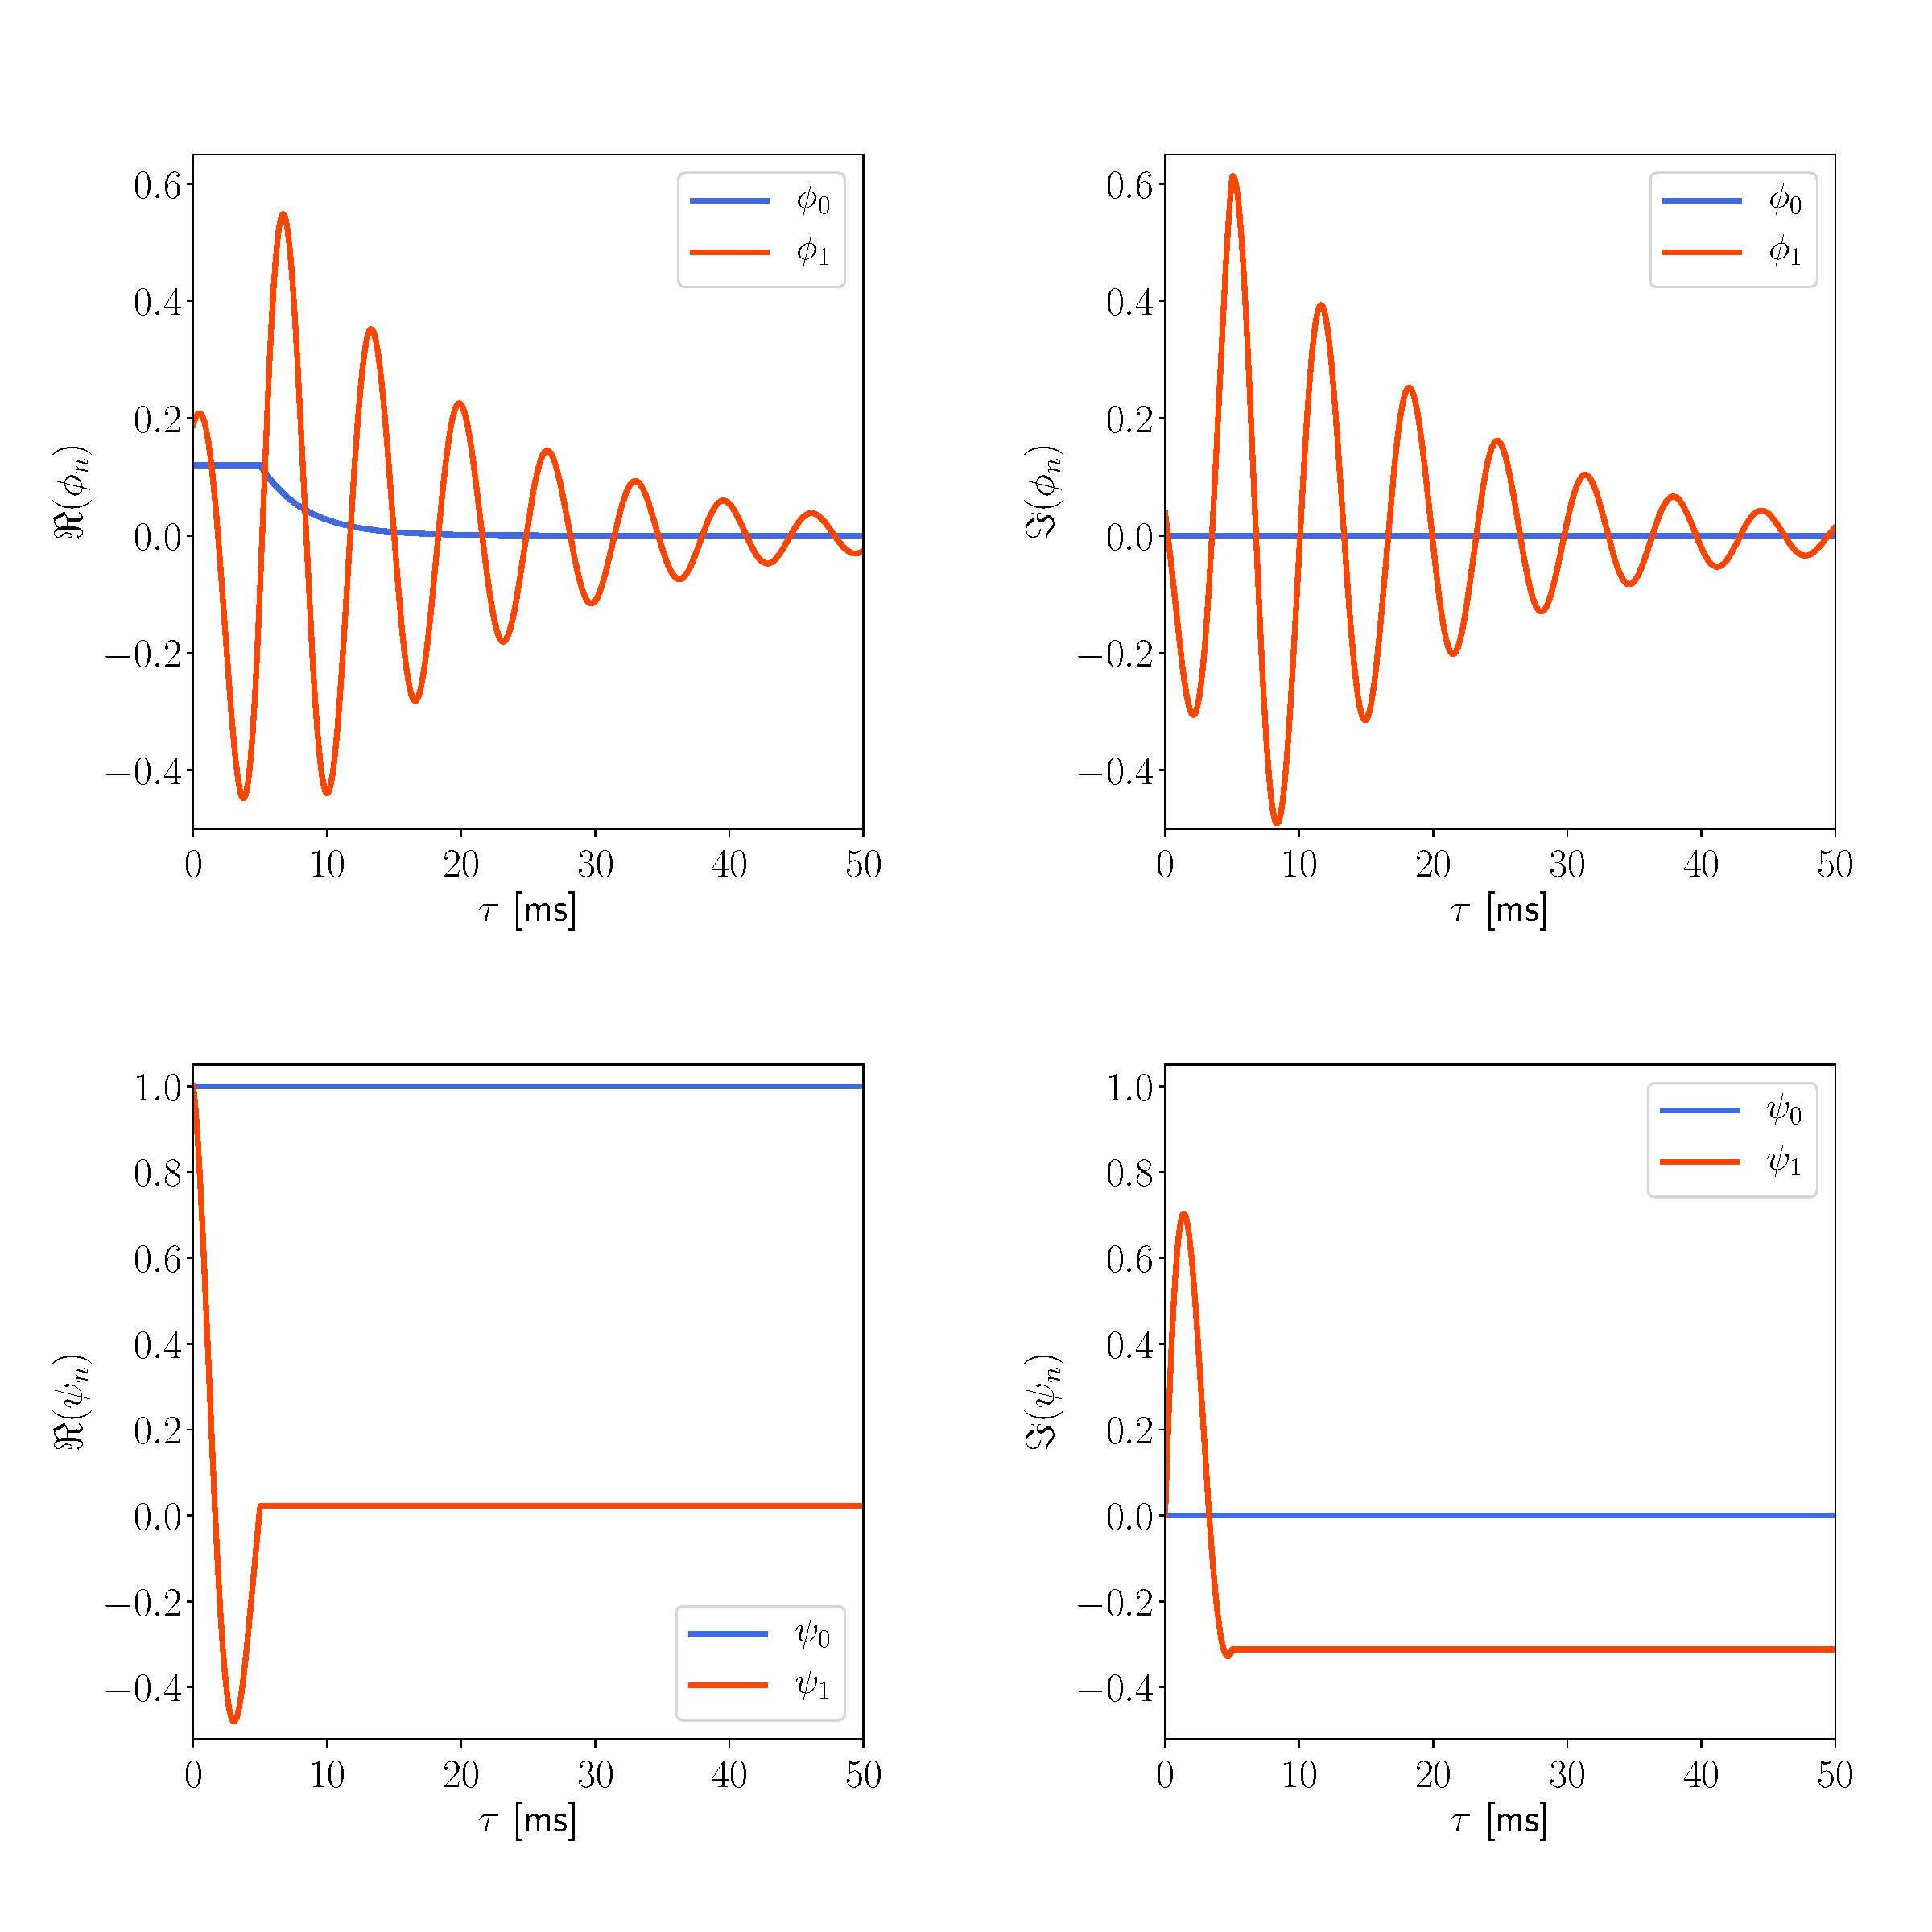
\includegraphics[width=0.8\linewidth]{poisson_eigenfunction.pdf}
	\caption{Real part (left) and imaginary part (right) of the eigenfunctions $\phi_n$ and $\psi_n$ of the first modes for Poisson neuron with absolute refractoriness $\Delta$, with $Delta=5$ ms, $h=h_0$, $\nu_{max}=0.6$ kHz. $\phi{-1}$ and $\psi_{-1}$  are the complex conjugate of respectively $\phi_{1}$ and $\psi_{-1}$ }
	\label{fig:poissoneigenfunction}
\end{figure}


\subsubsection{Gamma process}

Taking the Laplace transsform of the ISI density of a gamma process Eq. \eqref{eq:gamma} yields:

\begin{equation}
P_L(\lambda)=\big(\frac{\beta}{\beta +\lambda}\big)^\gamma
\end{equation}


The condition given by Eq.\eqref{eq:condition2} leads then to the solutions


\begin{equation}
\lambda_n=\beta(\exp(\frac{2\pi i}{\gamma}n)-1), \hspace{2.8cm}  n=0,..., \gamma-1
\end{equation}

This can be rewritten in function of the rate $R$ and the coefficient of variation $C_v$ as

\begin{equation}
\lambda_n=RC_V^{-2}(\exp(2\pi iC_V^2 n)-1)
\end{equation}

And Eq.\ref{eq:psi0} yields to
\begin{equation}
\phi_n(0)=\frac{1}{\gamma\beta^\gamma(\beta+\lambda_n)^{-(\gamma+1)}}
\end{equation}


\begin{figure}
	\centering
	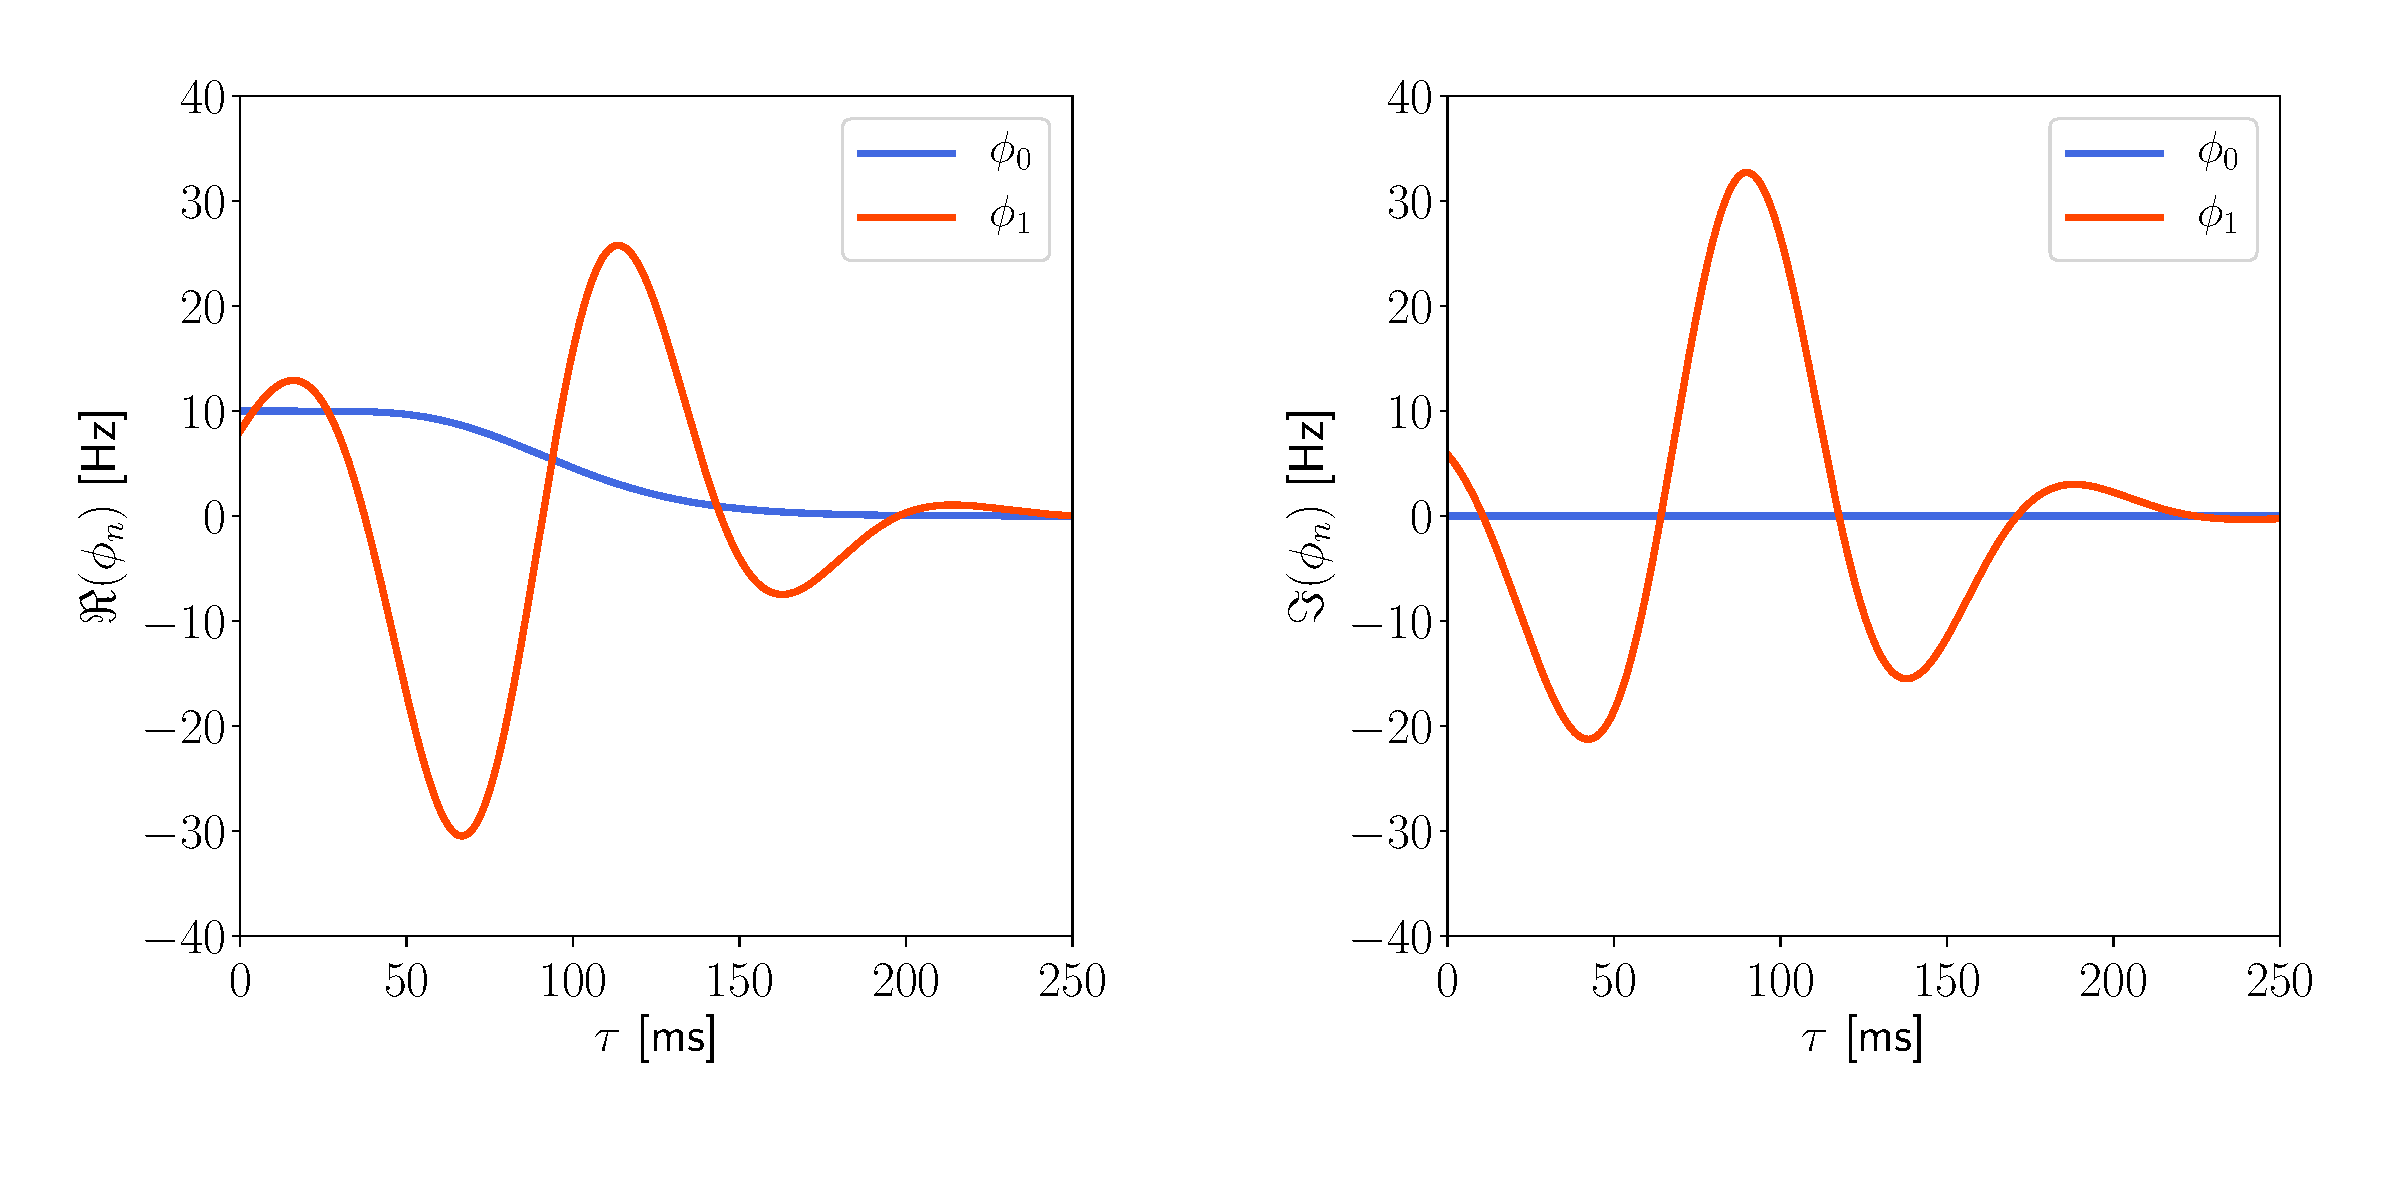
\includegraphics[width=0.8\linewidth]{gamma_eigenfunction.pdf}
	\caption{Real part (left) and imaginary part (right) of the eigenfunction $\phi_n$ of the first modes for a Gamma Process with $\beta=100$
		$\gamma=10$. $\phi{-1}$ is the complex conjugate of  $\phi_{1}$}
	\label{fig:gammaeigenfunction}
\end{figure}



\subsubsection{PIF neuron}

For a perfect integrating and  fire neuron the Laplace transsform of the ISI density Eq. \eqref{eq:iversegaussian} is

\begin{equation}
P_L(\lambda)=\exp\big(\frac{\mu V_{th}}{2D}\big[1-\sqrt{1+\frac{4D\lambda}{\mu^2}}\big]\big)
\end{equation}



The condition given by Eq.\eqref{eq:condition2} leads then to the solutions
\begin{equation}
 \lambda_n=- \frac{2\pi\mu}{V_{th}}n( \frac{2\pi D}{\mu V_{th}}n + i)
\end{equation}

The spectrum can be rewritten as a function of the rate $R$ and the coefficient of variation $C_v$

\begin{equation}
\lambda_n=- 2\pi^2R^2C_V^2n^2+2\pi R i\:n
\end{equation}

\subsection{A general approximation of the spectrum}

It is not always possible to analytically compute the Laplace transform $P_L(s)$ of a general ISI distribution $P(\tau)$. Thats why we would like to find a method to approximate the first eigenvalue $\lambda_1$. From Eq.\eqref{eq:Pmoment2} one can see that the the Laplace transform of ISI distribution can be rewritten with the cumulant $\kappa_n$ as:

\begin{equation}
\label{eq:PLcum}
P_L(\lambda)=\exp\left[ \sum_{k=1}^{+\infty}(-1)^k\kappa_k \frac{\lambda^k}{k!}\right]
\end{equation}

The condition Eq.\eqref{eq:condition2} can be then rewritten as:

\begin{equation}
\label{eq:cum2pi}
 \sum_{k=1}^{+\infty}(-1)^k\kappa_n \frac{\lambda_n^k}{k!}=2 \pi i n
\end{equation}

We can approximate teh first eigenvalue $\lambda_1$, keeping only the terms until the second cumulant, Eq.\eqref{eq:cum2pi} becomes

\begin{equation}
\label{eq:cumaprox}
\frac{\kappa_2}{2}\lambda_1^2-\kappa_1\lambda_1 -2\pi i
\end{equation}

$\lambda_1$ correspond to the roots of Eq.\eqref{eq:cumaprox} with the negative real parts, as we shown before a positive real part would be unphysical. The approximation of $\lambda_1$ can be rewritten in terms of the rate $R$ and the coefficient of variation $C_V$: 

\begin{equation}
\label{eq:l1aprox}
\lambda_1\simeq RC_V^{-2}\left( 1-\sqrt{1+4\pi i C_V^2}\right)
\end{equation}

In the schaffer paper to detremine the first eigenvalue $\lambda_1$ they fitted the real part and the imaginary part as a function of $R$ and $C_V^2$. They found as a relationship for small $C_V$:

\begin{equation}
\label{eqschaffer}
\lambda_1 \simeq -R\left( (\frac{C_V}{0.22})^2+2\pi i\right) 
\end{equation}

Note that for small $C_V$ we can expand taylor expand the square root and recover an expression close to Eq.\eqref{eqschaffer}

\begin{equation}
\label{eq:l1aprox2}
\lambda_1\simeq -R\left(2\pi^2 C_V^2+2\pi i\right) + \mathcal{O}(C_V^4)
\end{equation}




 



\section{General renewal neuron}
\label{sec:gen-renw}

\subsection{Population response to time-dependent input}

--for uncoupled neurons
--susceptibility

\section{Population dynamics of coupled neurons}

- one population

- two populations (E-I net)


\bibliography{my}




\end{document}